
Выберем 3 модели - линейная, логистическая и ridge регрессии, обучим на них классификатор и сравним качество

\begin{table}[h]
    \centering
    \label{tab:results}
    \begin{tabular}{cccccc}
    \toprule
    N & Модель & Precision & Accuracy & Recall \\
    \midrule
    \multirow{3}{*}{25} 
        & Logistic & 0.8071 & 0.8037 & 0.7980 \\
        & Linear & 0.8426 & 0.8077 & 0.7567 \\
        & Ridge & 0.8426 & 0.8077 & 0.7567 \\
    \hline
    \multirow{3}{*}{100} 
        & Logistic & 0.9700 & 0.9693 & 0.9687 \\
        & Linear & 0.9907 & 0.9597 & 0.9280 \\
        & Ridge & 0.9907 & 0.9597 & 0.9280 \\
    \hline
    \multirow{3}{*}{500} 
        & Logistic & 1.0000 & 0.9993 & 0.9987 \\
        & Linear & 1.0000 & 0.9993 & 0.9987 \\
        & Ridge & 1.0000 & 0.9993 & 0.9987 \\
    \bottomrule
    \end{tabular}
\end{table}

Все линейные модели дают очень близкий результат, поэтому зафиксируем в качестве модели обычную \textbf{логистическую регрессию}\\

\textbf{Проведем кроссвалидацию для оценки дисперсии метрик}\\

\hspace*{-1cm}
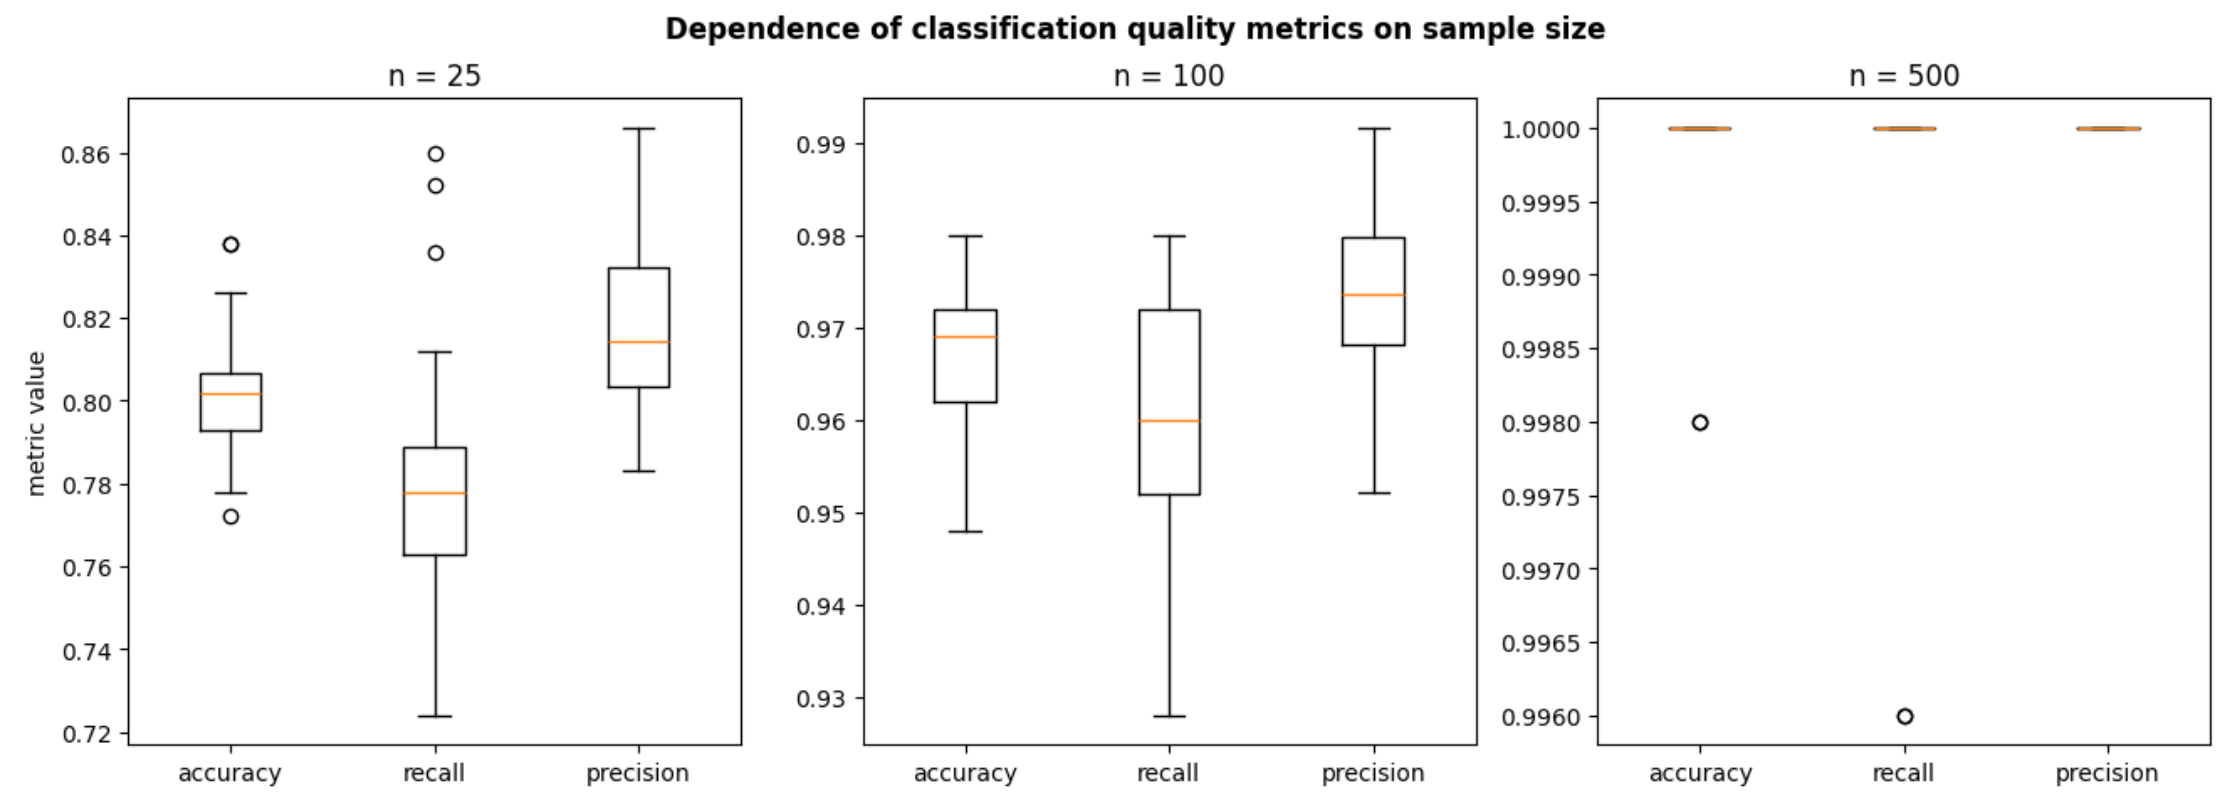
\includegraphics[width=1\textwidth]{Part-II_student-2/dependence metrics on sample size}\\ 

\textbf{Занесем данные в таблицу}\\

\begin{table}[h]
    \centering
    \begin{tabular}{lccc}
    \toprule
    \textbf{Размер выборки} & \textbf{Метрика} & \textbf{Среднее} & \textbf{Дисперсия} \\
    \midrule
    \multirow{3}{*}{N=25} 
     & Accuracy  & 0.80  & 0.000271 \\
     & Recall    & 0.78  & 0.001231 \\
     & Precision & 0.81  & 0.000460 \\
    \midrule
    \multirow{3}{*}{N=100}
     & Accuracy  & 0.97  & $6.384 \times 10^{-5}$ \\
     & Recall    & 0.96  & 0.000166 \\
     & Precision & 0.97  & $9.624 \times 10^{-5}$ \\
    \midrule
    \multirow{3}{*}{N=500}
     & Accuracy  & 0.999 & $3.6 \times 10^{-7}$ \\
     & Recall    & 0.999 & $1.44 \times 10^{-6}$ \\
     & Precision & 0.99  & 0.0 \\
    \bottomrule
    \end{tabular}
\end{table}

\noindent\textbf{Выводы:}
\begin{itemize}
    \item Увеличение выборки снижает дисперсию экспоненциально

    \item \textbf{Стабильность метрик:}
        \begin{itemize}
            \item Precision демонстрирует самую низкую дисперсию на всех выборках
            \item Recall наиболее чувствителен к размеру выборки

        \end{itemize}
    
    \item \textbf{Оптимальный размер:} Для данной задачи выборка размером n=100 уже обеспечивает отличные результаты, а дальнейшее увеличение (n=500) лишь незначительно улучшает метрики и их стабильность.
\end{itemize}

\restoregeometry